\chapter{Variabili Aleatorie}

\begin{figure}[H]
	\centering
	\caption{Tipi di variabili casuali}
	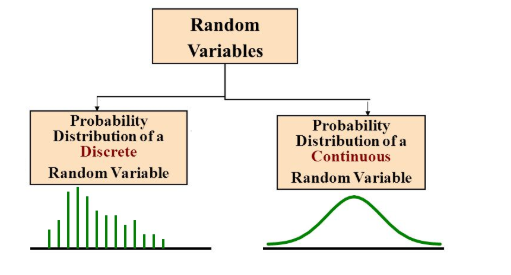
\includegraphics[]{varrandom}
\end{figure}

\section{Variabili Aleatorie Discrete}

Una variabile aleatoria (casuale o stocastica) discreta è una variabile che può assumere diversi valori in dipendenza da qualche fenomeno casuale.
Il risultato del lancio di un dado, ad esempio, è una variabile aleatoria discreta.

Prendiamo uno \textbf{spazio probabilizzabile} $ (\Omega, F) $ e una variabile aleatoria discreta $ x : \Omega \to \R $, che è una funzione continua non surgettiva. I valori di $ x $ devono essere un sottoinsieme finito di $ \R $ ovvero $ \{a_1, \dots, a_k\} $.
Vogliamo anche che $ \forall j \in [1, k] $ sia vero $ x^{-1}(a_j) = \{ \omega \in \Omega, x(\omega) = a_j\} \in F $. Utilizziamo la funzione inversa per ottenere gli elementi di $ \Omega $ su cui possiamo definire la probabilità.

Con la probabilità di tutti gli eventi definisco la densità di probabilità. Nello spazio probabilizzato $ (\Omega, F, \mathcal{P}) $ la probabilità che la variabile aleatoria assuma il valore $ a_j $ sarà $ p_j = \p{x = a_j} = \p{x^{-1}(a_j)} $, che viene detta densità di probabilità. Varranno quindi le seguenti proprietà

\begin{enumerate}
	\item $ \forall j \ldotp x^{-1} (a_j) $ sono tutti insiemi disgiunti.
	\item Essi coprono tutto $ \Omega $
\end{enumerate}

Vale che $ \sum_{j=1}^{k} p_j = 1 $. Poiché:
\[ 1 = \p{\Omega} = \p{\bigcup_{j} x^{-1}(a_j)} = \sum_{j} \p{x^{-1}(a_j)}\] 

Sia $ x : \Omega \to \{ a_1, \dots, a_k \} $ una variabile aleatoria, e sia la densità di probabilità $ p_j \geq 0 $ e anche  $ \sum_{j=1}^{k} p_j = 1 $, allora $ \p{x = a_j} = p_j $.

Preso uno spazio probabilizzabile $ (\Omega, F) $ e una variabile aleatoria $ x : \Omega \to \{ a_1, \dots, a_k \} $, supponendo che i numeri $ a_j $ siano ordinati, sia $ p_j $ la densità di probabilità, come posso ricostruire, ad esempio $ \p{x \leq a_3} $?

\[ \p{x \leq a_3} = \p{(x=a_1) \cup (x=a_2) \cup (x=a_3)} = \p{x = a_1} + \p{x = a_2} + \p{x = a_3}  \]

\paragraph{Esempio}

Voglio contare quanti 6 escono in 10 lanci di dadi.

Sia $ \Omega = \{ (1, 2, 3, 4, 5, 6)\}^{10} $, ovvero tutte le possibili parole di 10 elementi composte dai numeri da 1 a 6. Ad ogni lancio, ho $ \frac{1}{6} $ di probabilità di ottenere 6 e $ \frac{5}{6} $ di ottenere gli altri numeri. Definiamo la variabile aleatoria $ x : \Omega \to \{ 0, 1, 2, \dots, 9, 10 \} $ come il conteggio dei risultati dei lanci dove ottengo 6. Qual'è la probabilità di ottenere 3 lanci dove ho fatto 6?

\[ \p{x = 3} = \binom{10}{3} \left(\dfrac{1}{6}\right)^3 \left(\dfrac{5}{6}\right)^7 \]

% TODO spiega

\subsection{Legge di Bernoulli}
Faccio un esperimento, il risultato positivo ha probabilità $ p $, mentre il risultato negativo ha probabilità $ 1 - p $

Sia lo spazio $ \Omega = \begin{cases}
\text{successo} \to 1 \\
\text{insuccesso} \to 0
\end{cases} $

Una variabile aleatoria Bernoulliana è definita come $ x : \Omega \to \begin{cases}
p_1 = p \\ p_0 = 1 - p
\end{cases} $

\paragraph{Legge Binomiale} 
Sia $ k $ il conteggio dei successi di $ n $ esperimenti, abbiamo quindi che $ B(n,p) = x_i\{(0,1)\}^n \to \{0, \dots, n\} $. Abbiamo che la densità di probabilità Binomiale $ p_k = \p{x=k} = \binom{n}{k} p^k(1-p)^{n-k} $.

$ p_k $ è una densità? Sappiamo che $ p_k \geq 0 $ e sappiamo che $ 1 = \sum_{k} p_k $, con il binomio di Newton possiamo dimostrare che $ (a+b)^n = \sum_{k=0}^{n} \binom{n}{k} a^k b^{n-k} $. Proseguendo, abbiamo che 

\[ \sum_{k} p_k = \sum_{k=0}^{n} \binom{n}{k} p^k (1-p)^{n-k} = (p+(1-p)^n) = 1^n = 1 \]

\subsection{Somma di Variabili Aleatorie}
Lancio due dadi, uno rosso e uno nero, avremo quindi $ \Omega = \{R, N\} = \{(1,6)\}^2 $. Definisco due variabili aleatorie, $ x $ per il dado rosso dove $ x : (R, N) \to R $ e la variabile $ y : (R, N) \to N $. La densità per $ x $ sarà $ p_j = \frac{1}{6} \forall j $ mentre la densità per $ y $ sarà $ q_j = \frac{1}{6} \forall j $
Avremo che $ z = x + y $ conta la somma dei dadi.

\paragraph{Esercizi}
\begin{enumerate}
	\item Calcolare la densità di $ z $
		
		In questo caso $ x, y $ sono indipendenti, quindi avremo la densità di $ z $ detta $ t_z $.
		
		\[ \forall n \in [2, 12] .  \left( \p{z = n} = \sum_{i=1}^{n-1} \p{x = i} \cdot \p{y = n - i} \right) \]
		
		\begin{table}[H]
			\centering
			\caption{Distribuzione discreta della somma del lancio di due dadi.}
			\label{tab:distribdice1}
			\begin{tabular}{|l|l|l|l|l|l|l|l|l|l|l|l|}
				\hline
				$ x + y $     & 2        & 3        & 4        & 5        & 6        & 7        & 8        & 9        & 10       & 11       & 12       \\ \hline
				$ p_j + q_j $ & $ 1/36 $ & $ 2/36 $ & $ 3/36 $ & $ 4/36 $ & $ 5/36 $ & $ 6/36 $ & $ 5/36 $ & $ 4/36 $ & $ 3/36 $ & $ 2/36 $ & $ 1/36 $ \\ \hline
			\end{tabular}
		\end{table}
		
	\item Calcolare $ \p{4 \leq z \leq 6} $
	
	$ \p{4 \leq z \leq 6} = \p{4} + \p{5} + \p{6} = \frac{3}{36} + \frac{4}{36} + \frac{5}{36} = \frac{12}{36} = \frac{1}{3} $
\end{enumerate}

\begin{figure}[H]
	\centering
	\caption{Distribuzione della somma del lancio di due dadi}
	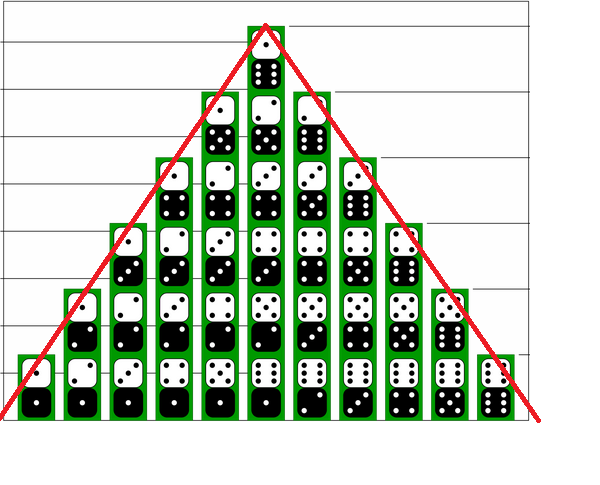
\includegraphics[]{binomdadi}
\end{figure}

% TODO Svolgi

\subsection{Indipendenza di Variabili Aleatorie}

Due variabili aleatorie $ x_1, x_2 $ sono indipendenti se $ \forall I_1, I_2, \subseteq \R $ intervalli o semirette si ha che 

\[ \left( \p{x_1 \in I_1} \cap \p{x_2 \in I_2} \right) = \p{x_1 \in I_1} - \p{x_2 \in I_2} \]

Nell'esempio di prima $ x, z $ e $ y,z $ sono dipendenti perché dati $ I_1 = [1,2], I_2 = [3,4] $ allora si ha che $ \p{x\in I_1} = \p{x=1,2} = \frac{1}{3} $ e si ha anche $ \p{z \in I_2} = \p{2 = 3,4} = \frac{5}{36} $. Ne otteniamo che:

% TODO fix erratum

\[ \p{(x \in I_1) \cap (z = 3,4)} = \p{(x = 1,2, z = 3,4)} = \dfrac{4}{12} \]

\paragraph{Variabili Aleatorie Congiunte}
Due variabili aleatorie $ x,y : \Omega \to \R $ discrete sono congiunte quando si può calcolare $ \p{x = m \cap y = n} = p_{n,m} $, ovvero una densità di probabilità $ \{ p_{n,m} \}_{n,m} $ con $ (p_{n,m} \geq 0 ) \land (\sum_{n,m} p_{n,m} = 1) $.

Sapendo $ p_{n,m} $ ricavo tutti i $ \p{x=m} = p_m $ e $ \p{y = n} = q_n $ con

\[ \p{x=m} = \p{x = m \cap \left\{ \bigcup_{n} y=n \right\}} = \sum_{n} \p{x=m,y=n} = \sum_n p_{n,m} = p_m \]
\[ \p{y=n} = \sum_{m} p_{n,m} = q_n \]

Non si può ricostruire dalle due probabilità la variabile aleatoria congiunta. Ad esempio, conoscendo $ p_n,q_n $ cerco $ p_n,m  = \p{x = m \cap y = n} = \p{x = m | y = n} \cdot \p{y=n} $. Se $ x,y $ sono indipendenti allora $ P(x=m|y=n) = \p{x=m} $ e vale il prodotto $ p_{m,n} = p_n \cdot p_m $.

\[ \sum_{m}\sum_{n} p_{n,m} = \sum_{m}\sum_{n} p_n \cdot q_n = \left( \sum_{m} p_m \right) \left( \sum_{n} q_m \right) = 1 \]

\paragraph{Formula di Convoluzione}

Tornando alla somma di due variabili aleatorie discrete, dati $ x,y $ indipendenti e $ z = x + y $, con $ x,y : \Omega \to \N $, dobbiamo calcolare $ \p{z = n} $ e la densità di probabilità discreta $ \left\{z = n\right\} $

\[ \left\{z = n\right\} = \bigcup_{i=0}^{n} \left\{x = 1 \cap y = n - i \right\} \]

\[ \p{z=n} = \sum_{i} \p{x = i \cap y = n-1} = \sum_{i = n}^{n} \p{x=i} \cdot \p{y=n-i} \]

\paragraph{Teorema: Rapporto fra Bernoulli e Binomiale}

Sommando $ n $ esperimenti di $ p $ dove conto i successi ottengo la binomiale $ B(n,p) $, quindi $ \sum_{i=1}^{n} \text{Bern}_i(p) = B(n,p) $

\paragraph{Dimostrazione per Induzione}
Caso base, per $ n = 1 \implies B(1,p) = \text{Bern}(p)$. Come passo induttivo abbiamo 
\[ B(n,p) = \sum_{i=1}^{n} \text{Bern}_i(p) \implies B(n+1,p) = \sum_{i=1}^{n+1} = \text{Bern}_i(p) \]
\[ \sum_{i=1}^{n+1} \text{Bern}_i(p) = \left( \sum_{i=1}^{n} \text{Bern}_i(p) \right) + \text{Bern}_{n+1}(p) = B)(n,p) + \text{Bern}(p) \]

Introduciamo le densità per continuare la dimostrazione
\[ \p{B(n,p) + \text{Bern}(p) = k} = \p{B(n,p) = k \cap \text{Bern}(p) = 0} + \p{B(n,p) = k-1 \cap \text{Bern}(p) = 1} \]
\[ = \binom{n}{k-1}p^{k-1}(1-p)^{n-k+1} \cdot p + \binom{n}{k}p^k(1-p)^{n-k} \cdot  (1-p) \]
\[ = \left[\binom{n}{k-1}\binom{n}{k}\right] p^k (1-p)^{n-k+1} = \binom{n+1}{k} p^k (1-p)^{n+1-k} = \p{B(n+1,p) = k}\]

\section{Variabile Geometrica}
Data una successione di esperimenti ripetuti con probabilità di successo $ 0 \leq p \leq 1 $. Lo ripeto fino ad ottenere un successo. $ \geom(p) $ conta il numero di prove necessarie. Ovvero $ \p{\geom(p) = k} = $ la probabilità di fare k esperimenti ed avere un successo dall'ultimo. La densità di probabilità sarà $ p_k = \p{\geom(p) = k} = (1-p)^{k-1} \cdot p $ con $ p_k \geq 0 $ e anche $ \sum_{k=1}^{\infty} (1-p)^{k-1} p = p \sum_{k=1}^{\infty}(1-p)^{k-1} $, che è una serie geometrica. Sarà quindi equivalente a $ p \sum_{i=0}^{n} (1-p)^i = \dfrac{p}{1-(1-p)} = 1$


Osservazione: consideriamo la serie geometrica $ \sum_{i=0}^{\infty} q^i $.
Sappiamo che $ (1-q) \sum_{i=0}^{\infty} q^i = 1 $ perché $ (1-q)(1+q+q^2+q^3\dots) $ = $( 1 - q + q - q^2 + q^2 + \dots )$, semplificando i termini rimane 1.

Una variabile geometrica \textbf{non ha memoria}, l'esperimento numero $ n $ ha la stessa probabilità degli altri esperimenti:

\[ \p{\geom(p) = n+m | \geom(p) > n} = \p{\geom(p) = m}  = \]
\[ = \dfrac{\p{\geom(p) = m + n \cap \geom(p) > n}}{\p{\geom(p) > n}} = \dfrac{\p{\geom(p) = m+n}}{\p{\geom(p) > n}}\] 
\[= \dfrac{(1-p)^{m+n-1} \cdot p}{(1-p)^n} = \p{\geom(p) = m} \]

Si può dimostrare sapendo che $ \forall m . \p{\geom(p) = n+m \cap \p{\geom} > n} = \p{\geom(p) = m+n} $

\subsection{Variabili Ipergeometriche}

Siano dati $ r $ sfere rosse, $ b $ sfere bianche, $ n $ estrazioni senza reimbussolamento, $ k = $ numero di sfere rosse estratte, $ H(b+r, r, n) $ conta il numero di sfere rosse estratte dopo n tentativi. Sappiamo che $ (0 < n \leq b + r) \land (k \leq n)  \land (k \leq r) \land (n-k \leq b) $.

Definiamo la densità di probabilità
\[ \p{H(b+r, r, n) = k} = \dfrac{\binom{r}{k} \binom{b}{n-k}}{\binom{b+r}{n}} \] 

\paragraph{Esercizio} Dati $ r = 10, 15 = b, 7 = n $ abbiamo che $ H(25,15,7) $

Esercizio per casa: $ \p{H(25, 15, 7) = 3} $